% Options for packages loaded elsewhere
\PassOptionsToPackage{unicode}{hyperref}
\PassOptionsToPackage{hyphens}{url}
\PassOptionsToPackage{dvipsnames,svgnames*,x11names*}{xcolor}
%
\documentclass[
  11pt,
]{krantz}
\usepackage{lmodern}
\usepackage{amssymb,amsmath}
\usepackage{ifxetex,ifluatex}
\ifnum 0\ifxetex 1\fi\ifluatex 1\fi=0 % if pdftex
  \usepackage[T1]{fontenc}
  \usepackage[utf8]{inputenc}
  \usepackage{textcomp} % provide euro and other symbols
\else % if luatex or xetex
  \usepackage{unicode-math}
  \defaultfontfeatures{Scale=MatchLowercase}
  \defaultfontfeatures[\rmfamily]{Ligatures=TeX,Scale=1}
\fi
% Use upquote if available, for straight quotes in verbatim environments
\IfFileExists{upquote.sty}{\usepackage{upquote}}{}
\IfFileExists{microtype.sty}{% use microtype if available
  \usepackage[]{microtype}
  \UseMicrotypeSet[protrusion]{basicmath} % disable protrusion for tt fonts
}{}
\makeatletter
\@ifundefined{KOMAClassName}{% if non-KOMA class
  \IfFileExists{parskip.sty}{%
    \usepackage{parskip}
  }{% else
    \setlength{\parindent}{0pt}
    \setlength{\parskip}{6pt plus 2pt minus 1pt}}
}{% if KOMA class
  \KOMAoptions{parskip=half}}
\makeatother
\usepackage{xcolor}
\IfFileExists{xurl.sty}{\usepackage{xurl}}{} % add URL line breaks if available
\IfFileExists{bookmark.sty}{\usepackage{bookmark}}{\usepackage{hyperref}}
\hypersetup{
  pdftitle={통계 프로그래밍 언어},
  pdfauthor={한국한의학연구원, 구본초},
  colorlinks=true,
  linkcolor=Maroon,
  filecolor=Maroon,
  citecolor=Blue,
  urlcolor=Blue,
  pdfcreator={LaTeX via pandoc}}
\urlstyle{same} % disable monospaced font for URLs
\usepackage{color}
\usepackage{fancyvrb}
\newcommand{\VerbBar}{|}
\newcommand{\VERB}{\Verb[commandchars=\\\{\}]}
\DefineVerbatimEnvironment{Highlighting}{Verbatim}{commandchars=\\\{\}}
% Add ',fontsize=\small' for more characters per line
\usepackage{framed}
\definecolor{shadecolor}{RGB}{248,248,248}
\newenvironment{Shaded}{\begin{snugshade}}{\end{snugshade}}
\newcommand{\AlertTok}[1]{\textcolor[rgb]{0.33,0.33,0.33}{#1}}
\newcommand{\AnnotationTok}[1]{\textcolor[rgb]{0.37,0.37,0.37}{\textbf{\textit{#1}}}}
\newcommand{\AttributeTok}[1]{\textcolor[rgb]{0.61,0.61,0.61}{#1}}
\newcommand{\BaseNTok}[1]{\textcolor[rgb]{0.06,0.06,0.06}{#1}}
\newcommand{\BuiltInTok}[1]{#1}
\newcommand{\CharTok}[1]{\textcolor[rgb]{0.5,0.5,0.5}{#1}}
\newcommand{\CommentTok}[1]{\textcolor[rgb]{0.37,0.37,0.37}{\textit{#1}}}
\newcommand{\CommentVarTok}[1]{\textcolor[rgb]{0.37,0.37,0.37}{\textbf{\textit{#1}}}}
\newcommand{\ConstantTok}[1]{\textcolor[rgb]{0,0,0}{#1}}
\newcommand{\ControlFlowTok}[1]{\textcolor[rgb]{0.27,0.27,0.27}{\textbf{#1}}}
\newcommand{\DataTypeTok}[1]{\textcolor[rgb]{0.27,0.27,0.27}{#1}}
\newcommand{\DecValTok}[1]{\textcolor[rgb]{0.06,0.06,0.06}{#1}}
\newcommand{\DocumentationTok}[1]{\textcolor[rgb]{0.37,0.37,0.37}{\textbf{\textit{#1}}}}
\newcommand{\ErrorTok}[1]{\textcolor[rgb]{0.14,0.14,0.14}{\textbf{#1}}}
\newcommand{\ExtensionTok}[1]{#1}
\newcommand{\FloatTok}[1]{\textcolor[rgb]{0.06,0.06,0.06}{#1}}
\newcommand{\FunctionTok}[1]{\textcolor[rgb]{0,0,0}{#1}}
\newcommand{\ImportTok}[1]{#1}
\newcommand{\InformationTok}[1]{\textcolor[rgb]{0.37,0.37,0.37}{\textbf{\textit{#1}}}}
\newcommand{\KeywordTok}[1]{\textcolor[rgb]{0.27,0.27,0.27}{\textbf{#1}}}
\newcommand{\NormalTok}[1]{#1}
\newcommand{\OperatorTok}[1]{\textcolor[rgb]{0.43,0.43,0.43}{\textbf{#1}}}
\newcommand{\OtherTok}[1]{\textcolor[rgb]{0.37,0.37,0.37}{#1}}
\newcommand{\PreprocessorTok}[1]{\textcolor[rgb]{0.37,0.37,0.37}{\textit{#1}}}
\newcommand{\RegionMarkerTok}[1]{#1}
\newcommand{\SpecialCharTok}[1]{\textcolor[rgb]{0,0,0}{#1}}
\newcommand{\SpecialStringTok}[1]{\textcolor[rgb]{0.5,0.5,0.5}{#1}}
\newcommand{\StringTok}[1]{\textcolor[rgb]{0.5,0.5,0.5}{#1}}
\newcommand{\VariableTok}[1]{\textcolor[rgb]{0,0,0}{#1}}
\newcommand{\VerbatimStringTok}[1]{\textcolor[rgb]{0.5,0.5,0.5}{#1}}
\newcommand{\WarningTok}[1]{\textcolor[rgb]{0.37,0.37,0.37}{\textbf{\textit{#1}}}}
\usepackage{longtable,booktabs}
% Correct order of tables after \paragraph or \subparagraph
\usepackage{etoolbox}
\makeatletter
\patchcmd\longtable{\par}{\if@noskipsec\mbox{}\fi\par}{}{}
\makeatother
% Allow footnotes in longtable head/foot
\IfFileExists{footnotehyper.sty}{\usepackage{footnotehyper}}{\usepackage{footnote}}
\makesavenoteenv{longtable}
\usepackage{graphicx,grffile}
\makeatletter
\def\maxwidth{\ifdim\Gin@nat@width>\linewidth\linewidth\else\Gin@nat@width\fi}
\def\maxheight{\ifdim\Gin@nat@height>\textheight\textheight\else\Gin@nat@height\fi}
\makeatother
% Scale images if necessary, so that they will not overflow the page
% margins by default, and it is still possible to overwrite the defaults
% using explicit options in \includegraphics[width, height, ...]{}
\setkeys{Gin}{width=\maxwidth,height=\maxheight,keepaspectratio}
% Set default figure placement to htbp
\makeatletter
\def\fps@figure{htbp}
\makeatother
\setlength{\emergencystretch}{3em} % prevent overfull lines
\providecommand{\tightlist}{%
  \setlength{\itemsep}{0pt}\setlength{\parskip}{0pt}}
\setcounter{secnumdepth}{5}
\usepackage{kotex}
\usepackage{dhucs-cmap}
\usepackage{booktabs}
\usepackage{placeins}
\usepackage{enumerate}
\usepackage{amssymb}
\usepackage{amsmath}
\usepackage{mathtools}
\usepackage{float}
% \usepackage{setspace} \doublespacing
\usepackage{relsize}
\usepackage{bigints}
\usepackage{bm}
\usepackage{amsmath}
% \usepackage{titlesec}
\usepackage{lipsum}
\usepackage{longtable}
 \usepackage[font=small,labelfont=bf]{caption}
\usepackage{dcolumn}
\usepackage{array}
\usepackage{gensymb}
\usepackage{makecell}
\usepackage{multirow}
\usepackage{natbib}
\usepackage{rotating}
\usepackage[most]{tcolorbox}

\renewcommand\theadalign{cb}
\renewcommand\theadfont{\bfseries}
\renewcommand\theadgape{\Gape[4pt]}
\renewcommand\cellgape{\Gape[4pt]}
\DeclareMathAlphabet{\mathpzc}{OT1}{pzc}{m}{it}

\renewcommand\theadalign{cb}
\renewcommand\theadfont{\bfseries}
\renewcommand\theadgape{\Gape[4pt]}
\renewcommand\cellgape{\Gape[4pt]}

\newcolumntype{L}[1]{>{\raggedright\let\newline\\
\arraybackslash\hspace{0pt}}m{#1}}
\newcolumntype{C}[1]{>{\centering\let\newline\\
\arraybackslash\hspace{0pt}}m{#1}}
\newcolumntype{R}[1]{>{\raggedleft\let\newline\\
\arraybackslash\hspace{0pt}}m{#1}}
\newcolumntype{P}[1]{>{\raggedright\tabularxbackslash}p{#1}}
\newcommand{\specialcell}[2][c]{%
  \begin{tabular}[#1]{@{}c@{}}#2\end{tabular}}
\newcommand{\specialcelll}[2][l]{%
  \begin{tabular}[#1]{@{}l@{}}#2\end{tabular}}

\captionsetup[table]{aboveskip=0pt}
\captionsetup[table]{belowskip=10pt}

\linespread{1.5}

% \setmainfont[UprightFeatures={SmallCapsFont=AlegreyaSC-Regular}]{Alegreya}

\usepackage{framed,color}
\definecolor{shadecolor}{RGB}{248,248,248}

\renewcommand{\textfraction}{0.05}
\renewcommand{\topfraction}{0.8}
\renewcommand{\bottomfraction}{0.8}
\renewcommand{\floatpagefraction}{0.75}

% \renewenvironment{quote}{\begin{VF}}{\end{VF}}
\let\oldhref\href
\renewcommand{\href}[2]{#2\footnote{\url{#1}}}

\ifxetex
  \usepackage{letltxmacro}
  \setlength{\XeTeXLinkMargin}{1pt}
  \LetLtxMacro\SavedIncludeGraphics\includegraphics
  \def\includegraphics#1#{% #1 catches optional stuff (star/opt. arg.)
    \IncludeGraphicsAux{#1}%
  }%
  \newcommand*{\IncludeGraphicsAux}[2]{%
    \XeTeXLinkBox{%
      \SavedIncludeGraphics#1{#2}%
    }%
  }%
\fi

\makeatletter
\newenvironment{kframe}{%
\medskip{}
\setlength{\fboxsep}{.8em}
 \def\at@end@of@kframe{}%
 \ifinner\ifhmode%
  \def\at@end@of@kframe{\end{minipage}}%
  \begin{minipage}{\columnwidth}%
 \fi\fi%
 \def\FrameCommand##1{\hskip\@totalleftmargin \hskip-\fboxsep
 \colorbox{shadecolor}{##1}\hskip-\fboxsep
     % There is no \\@totalrightmargin, so:
     \hskip-\linewidth \hskip-\@totalleftmargin \hskip\columnwidth}%
 \MakeFramed {\advance\hsize-\width
   \@totalleftmargin\z@ \linewidth\hsize
   \@setminipage}}%
 {\par\unskip\endMakeFramed%
 \at@end@of@kframe}
\makeatother

\makeatletter
\@ifundefined{Shaded}{
}{\renewenvironment{Shaded}{\begin{kframe}}{\end{kframe}}}
\makeatother

\newenvironment{rmdblock}[1]
  {
  \begin{itemize}
  \renewcommand{\labelitemi}{
    \raisebox{-.7\height}[0pt][0pt]{
      {\setkeys{Gin}{width=3em,keepaspectratio}\includegraphics{images/#1}}
    }
  }
  \setlength{\fboxsep}{1em}
  \begin{kframe}
  \item
  }
  {
  \end{kframe}
  \end{itemize}
  }
  
\newenvironment{rmdnote}
  {\begin{rmdblock}{note}}
  {\end{rmdblock}}
  
\newenvironment{rmdcaution}
  {\begin{rmdblock}{caution}}
  {\end{rmdblock}}
  
\newenvironment{rmdimportant}
  {\begin{rmdblock}{important}}
  {\end{rmdblock}}
  
\newenvironment{rmdtip}
  {\begin{rmdblock}{tip}}
  {\end{rmdblock}}
  
\newenvironment{rmdwarning}
  {\begin{rmdblock}{warning}}
  {\end{rmdblock}}

\renewenvironment{quote}{\begin{kframe}}{\end{kframe}}

% \newenvironment{quoteshade}
%   {
%   \begin{itemize}
%   \begin{kframe}
%   \item
%   }
%   {
%   \end{kframe}
%   \end{itemize}
%   }
%   
% \newenvironment{rmdquote}
%  {\begin{quoteshade}}
%  {\end{quoteshade}}

\usepackage{makeidx}
\makeindex

\urlstyle{tt}

\usepackage{amsthm}
\makeatletter
\def\thm@space@setup{%
  \thm@preskip=8pt plus 2pt minus 4pt
  \thm@postskip=\thm@preskip
}
\makeatother

\frontmatter
\usepackage{booktabs}
\usepackage{longtable}
\usepackage{array}
\usepackage{multirow}
\usepackage{wrapfig}
\usepackage{float}
\usepackage{colortbl}
\usepackage{pdflscape}
\usepackage{tabu}
\usepackage{threeparttable}
\usepackage{threeparttablex}
\usepackage[normalem]{ulem}
\usepackage{makecell}
\usepackage{xcolor}
\usepackage[]{natbib}
\bibliographystyle{apalike}

\title{통계 프로그래밍 언어}
\author{한국한의학연구원, 구본초}
\date{2020-03-16}

\let\BeginKnitrBlock\begin \let\EndKnitrBlock\end
\begin{document}
\maketitle

{
\hypersetup{linkcolor=}
\setcounter{tocdepth}{2}
\tableofcontents
}
\listoftables
\listoffigures
\hypertarget{overview}{%
\chapter*{Course Overview}\label{overview}}


\BeginKnitrBlock{rmdnote}
본 문서는 2020년도 1학기 정보통계학과에서 개설한 ``통계 프로그래밍 언어'' 강의를 위해 개발한 강의 노트이며, Yihui Xie가 개발한 \textbf{bookdown} 패키지 \citep{R-bookdown}를 활용하여 생성한 문서이고 Google Chrome 또는 Firefox 브라우저에 최적화 됨. 아울러 충남대학교 정보통계학과 이상인 교수님의 2019년도 2학기 ``통계패키지활용'' 강의 노트와 동국대학교 ICT빅데이터학부 김진석 교수님의 \href{http://datamining.dongguk.ac.kr/lectures/R/_book/index.html}{R 프로그래밍 및 실습} 강의 자료 내용을 본 강의노트 작성에 참고함.

본 강의 노트는 주 단위로 업데이트될 예정이며, \url{https://zorba78.github.io/cnu-r-programming-lecture-note/} 에서 확인할 수 있고, 해당 페이지에서 pdf 파일 다운로드가 가능함.
\EndKnitrBlock{rmdnote}

\hypertarget{intro-lec}{%
\subsection*{강의소개}\label{intro-lec}}


R은 뉴질랜드 오클랜드 대학의 Robert Gentleman 과 Ross Ihaka 가 AT\&T 벨 연구소에서 개발한 S 언어를 기반으로 개발한 GNU 환경의 통계 계산 및 프로그래밍 언어이다. 현재 R 소프트웨어는 통계학 뿐 아니라 데이터 과학을 포함한 의학, 생물학 등 다양한 분야에서 활용되고 있으며 특히 통계 소프트웨어 개발과 데이터 분석에 많이 활용되고 있다. 본 강의는 데이터 분석을 위한 R의 기초 문법과 통계학 입문에서 학습한 몇 가지 중요한 통계적 이론에 대한 시뮬레이션 방법을 다룬다. 아울러 R package를 활용한 데이터 헨들링 및 시각화 그리고 Rmarkdown을 활용한 재현가능(reproducible)한 문서 작성법에 대해 학습하고자 한다.

\hypertarget{purpose-course}{%
\subsection*{교과 목표}\label{purpose-course}}


\begin{quote}
\begin{itemize}
\tightlist
\item
  \textbf{R 기초 문법 습득}
\item
  \textbf{R package를 활용한 데이터 핸들링 및 자료 시각화}
\item
  \textbf{R 시뮬레이션을 통한 통계학 기초 이론 확인}
\item
  \textbf{R을 이용한 데이터 분석 실습}
\item
  \textbf{R markdown을 이용한 재현가능(reproducible)한 보고서 작성 방법 습득}
\end{itemize}
\end{quote}

\hypertarget{pre-course}{%
\subsection*{선수과목}\label{pre-course}}


\begin{quote}
\textbf{통계학 개론}
\end{quote}

\hypertarget{course-method}
\item
  \textbf{실험/실습: 50\%}
\end{itemize}

\hypertarget{grade-method}
\item
  \textbf{기말고사: 40 \%}
\item
  \textbf{출석: 10 \%}
\item
  \textbf{과제: 10 \%}
\end{itemize}
\end{quote}

\hypertarget{policy-course}{%
\subsection*{수업 규정}\label{policy-course}}


\begin{quote}
\begin{itemize}
\tightlist
\item
  3번 지각은 1번 결석으로 처리
\item
  특별한 사유 없이 수업 중간에 이탈한 경우 결석으로 처리
\item
  특별한 사유로 인해 결석 또는 지각을 할 경우 사유를 증빙할 수 있는 서류 제출 시 출석으로 인정
\item
  출결 미달, 중간 또는 기말고사 미 응시인 경우 F 학점으로 처리
\item
  수업 중 휴대폰 및 각종 모바일 기기 사용 금지
\end{itemize}
\end{quote}

\hypertarget{material-course}{%
\subsection*{교재 및 참고문헌}\label{material-course}}


\begin{quote}
별도의 교재 없이 본 강의 노트로 수업을 진행할 예정이며, 수업의 이해도 향상을 위해 아래 소개할 도서 및 웹 문서 등을 참고할 것을 권장함.
\end{quote}

\textbf{참고 자료}

\begin{itemize}
\tightlist
\item
  실리콘밸리 데이터과학자가 알려주는 따라하며 배우는 데이터 과학 \citep{kwon-2017}
\item
  R을 이용한 데이터 처리\&분석 \citep{seo-2014}
\item
  R 그래픽스 \citep{ryu-2005}
\item
  \href{https://ggplot2-book.org/}{ggplot2: elegant graphics for data analysis} \citep{wickham-2016}
\item
  \href{https://r4ds.had.co.nz/}{R for data science} \citep{wickham-2016r}
\item
  Statistical Computing with R \citep{rizzo-2019}
\end{itemize}

\hypertarget{course-schedule}{%
\subsection*{강의 계획}\label{course-schedule}}


\begin{table}[H]

\caption{\label{tab:make-schedule-tab}강의 계획표}
\centering
\fontsize{10}{12}\selectfont
\begin{tabular}[t]{c>{\raggedright\arraybackslash}p{6cm}c}
\toprule
주차 & 강의 내용 & 과제\\
\midrule
\rowcolor{gray!6}  Week 1 & R 소개, R/R Studio 설치, R 패키지 설치, R 맛보기 및 markdown 문서 만들기 & 과제 1\\
Week 2 & R 자료형: 스칼라, 벡터, 리스트 & \\
\rowcolor{gray!6}  Week 3 & R 자료형: 행렬 및 배열 & 과제 2\\
Week 4 & R 자료형: 팩터, 테이블, 데이터 프레임 & \\
\rowcolor{gray!6}  Week 5 & R 자료형: 문자열과 정규 표현식 & 과제 3\\
\addlinespace
Week 6 & 데이터 프레임 가공 및 시각화 I & \\
\rowcolor{gray!6}  Week 7 & 데이터 프레임 가공 및 시각화 II & 과제 4\\
Week 8 & 중간고사 & \\
\rowcolor{gray!6}  Week 9 & 데이터 프레임 가공 및 시각화 III & \\
Week 10 & R 프로그래밍: 조건문, 반복문, 함수 & 과제 5\\
\addlinespace
\rowcolor{gray!6}  Week 11 & 통계시뮬레이션 I: 표본분포 및 중심극한정리 & \\
Week 12 & 통계시뮬레이션 2: 신뢰구간과 가설검정 & 과제 6\\
\rowcolor{gray!6}  Week 13 & R을 이용한 기초통계 분석 & \\
Week 14 & R markdown 활용 & 과제 7\\
\rowcolor{gray!6}  Week 15 & 기말고사 & \\
\bottomrule
\end{tabular}
\end{table}

\mainmatter

\hypertarget{part-get-started}{%
\part{Get Started}\label{part-get-started}}

\hypertarget{intro-chap}{%
\chapter{Introduction}\label{intro-chap}}

\textbf{1. R프로그램}

\begin{itemize}
\tightlist
\item
  데이터 분석을 위한 자료 전처리, 통계 및 시각화를 지원하는 컴퓨터 언어 및 환경
\item
  1980년 AT\&T 벨 연구소의 John Chambers가 개발한 S 언어를 기반으로 1995년 뉴질랜드 Auckland 대학의 통계학과 교수 Robert Gentleman과 Ross Ihaka 가 개발
\item
  \href{https://en.wikipedia.org/wiki/GNU_Project}{GNU} 기반의 오픈 소스
\item
  통계학, 전산학, 생물학, 의학 등 거의 모든 학문분야에서 분석도구로 활용되고 있고, 최근 data science 분야에서 널리 활용
\end{itemize}

\textbf{2. R 언어의 특징}

\begin{itemize}
\tightlist
\item
  \textbf{무료 소프트웨어}
\item
  \href{http://cran.r-project.org/web/view}{CRAN (Comprehensive R Archive Network)}에서 배포
\item
  특정 vendor가 아닌 전 세계 연구자들이 개발한 알고리즘 및 최신 함수 활용 가능(packaging system)
\item
  범용적으로 사용되는 거의 대부분의 운영체제(Windows, Mac, Linux)에서 작동 가능
\item
  방대한 개발 및 사용 생태계 형성
\item
  강력한 그래픽 기능
\end{itemize}

\footnotesize

\BeginKnitrBlock{rmdtip}
\textbf{유용한 웹 사이트}: R과 관련한 거의 모든 문제는 Googling (구글을 이용한 검색)을 통해 해결 가능(검색주제 + ``in R'' or ``in R software'')하고 많은 해답들이 아래 열거한 웹 페이지에 게시되어 있음.

\begin{itemize}
\tightlist
\item
  R 프로그래밍에 대한 Q\&A: \href{https://stackoverflow.com}{Stack Overflow}
\item
  R 관련 웹 문서 모음: \href{https://rpubs.com/}{Rpubs}
\item
  R package에 대한 raw source code 제공: \href{https://github.com}{Github}
\item
  R을 이용한 통계 분석: \href{http://www.sthda.com/english/}{Statistical tools for high-throughput data analysis (STHDA)}
\end{itemize}
\EndKnitrBlock{rmdtip}

\normalsize

\hypertarget{installation}{%
\section{R 설치하기}\label{installation}}

R 다운로드 사이트: \url{https://www.r-project.org} 또는 \url{https://cran.r-project.org}

\begin{enumerate}
\def\labelenumi{\arabic{enumi}.}
\item
  웹 브라우저(i.e.~Explore, Chrome, Firefox 등)의 주소 입력창에 \url{https://www.r-project.org}
\item
  좌측 R Logo 하단 Download 아래 CRAN 클릭
\end{enumerate}

\footnotesize

\begin{center}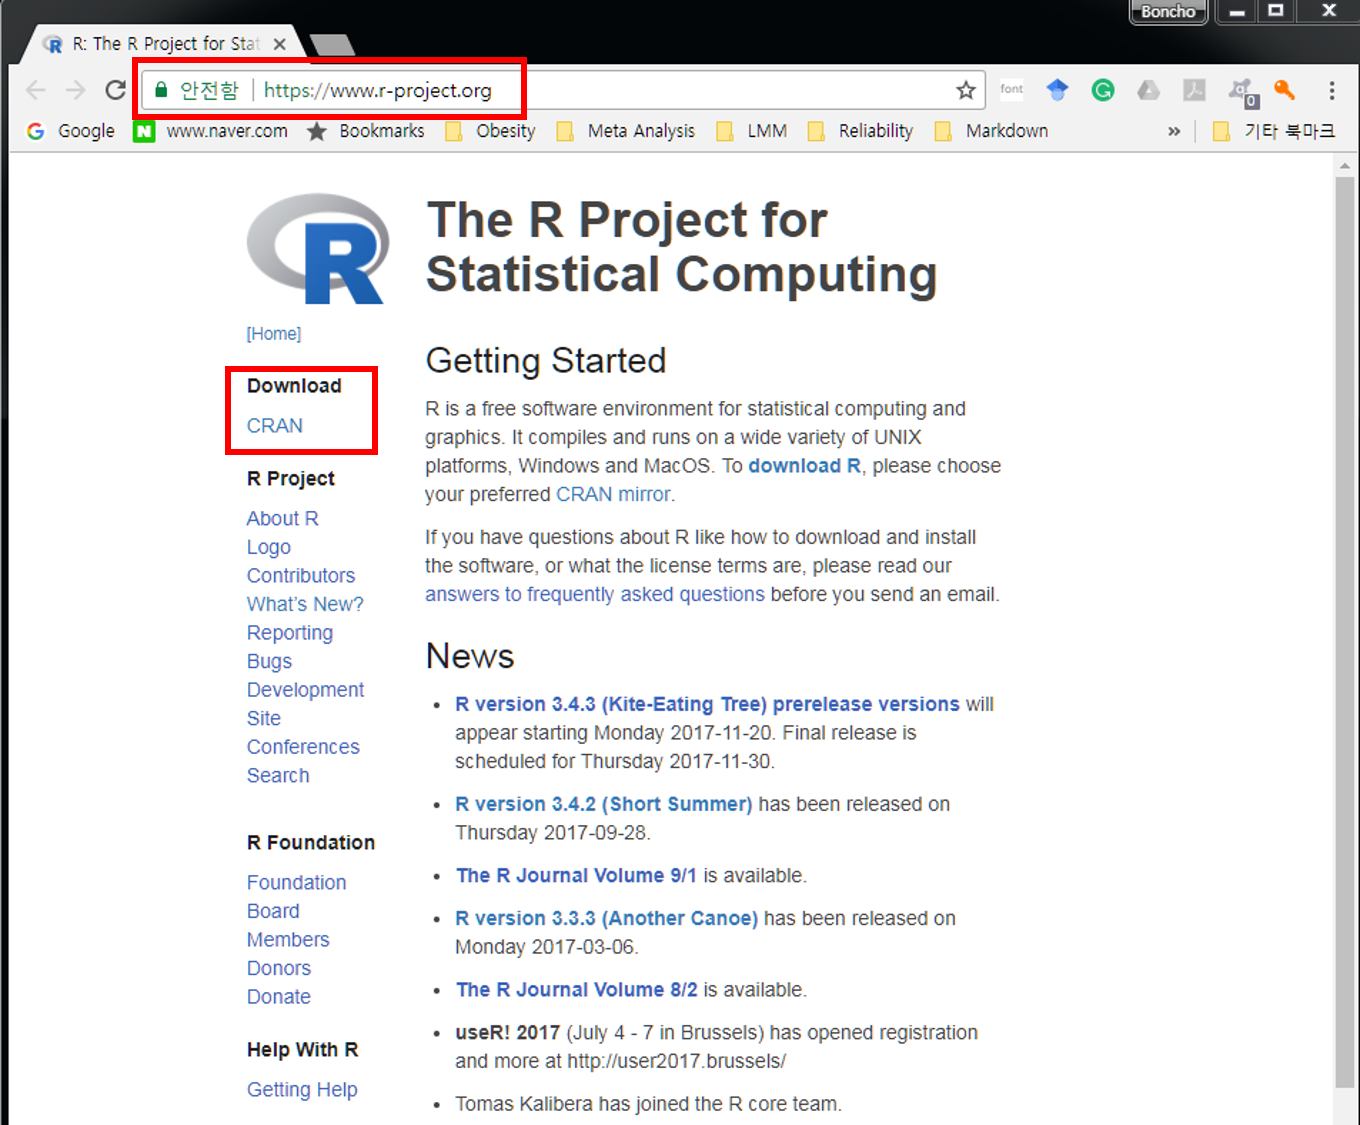
\includegraphics[width=0.9\linewidth]{figures/Rorg-main-add} \end{center}

\normalsize

\begin{enumerate}
\def\labelenumi{\arabic{enumi}.}
\setcounter{enumi}{2}
\tightlist
\item
  클릭 후 연결한 페이지를 스크롤 후 Korea 아래 링크\footnote{해당 링크들은 접속 시점에 따라 변경될 수 있음} 클릭
\end{enumerate}

\footnotesize

\begin{center}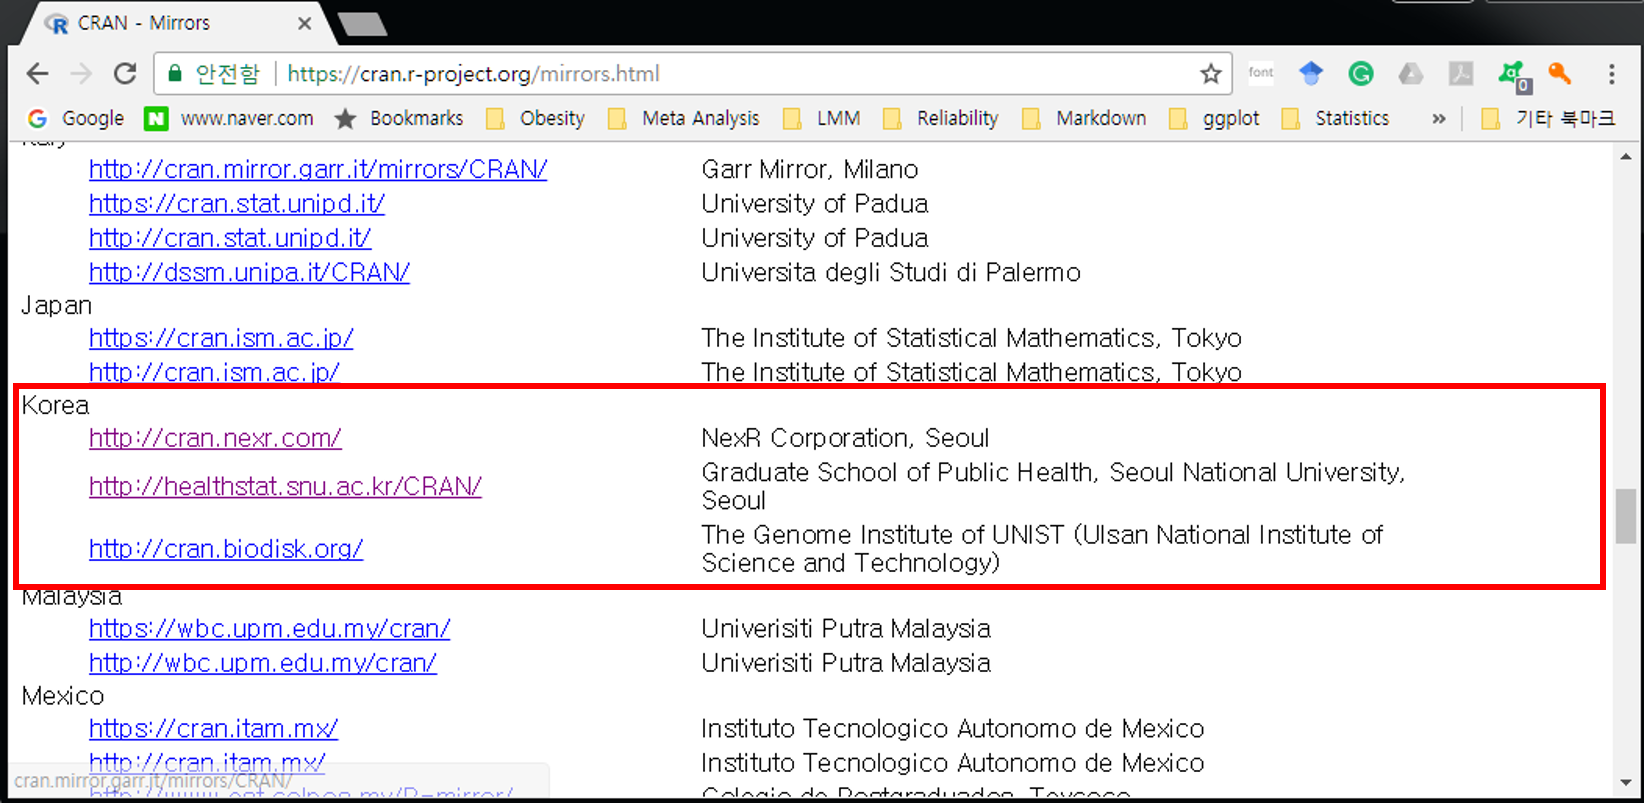
\includegraphics[width=0.9\linewidth]{figures/CRAN-korea-01} \end{center}

\normalsize

\begin{enumerate}
\def\labelenumi{\arabic{enumi}.}
\setcounter{enumi}{3}
\tightlist
\item
  클릭 후 세 가지 운영체제(Linux, Mac OS X, Windowns)에 따른 R 버전 선택 가능\footnote{본 노트는 Windows 버전 설치만 다룸}
\end{enumerate}

\footnotesize

\begin{center}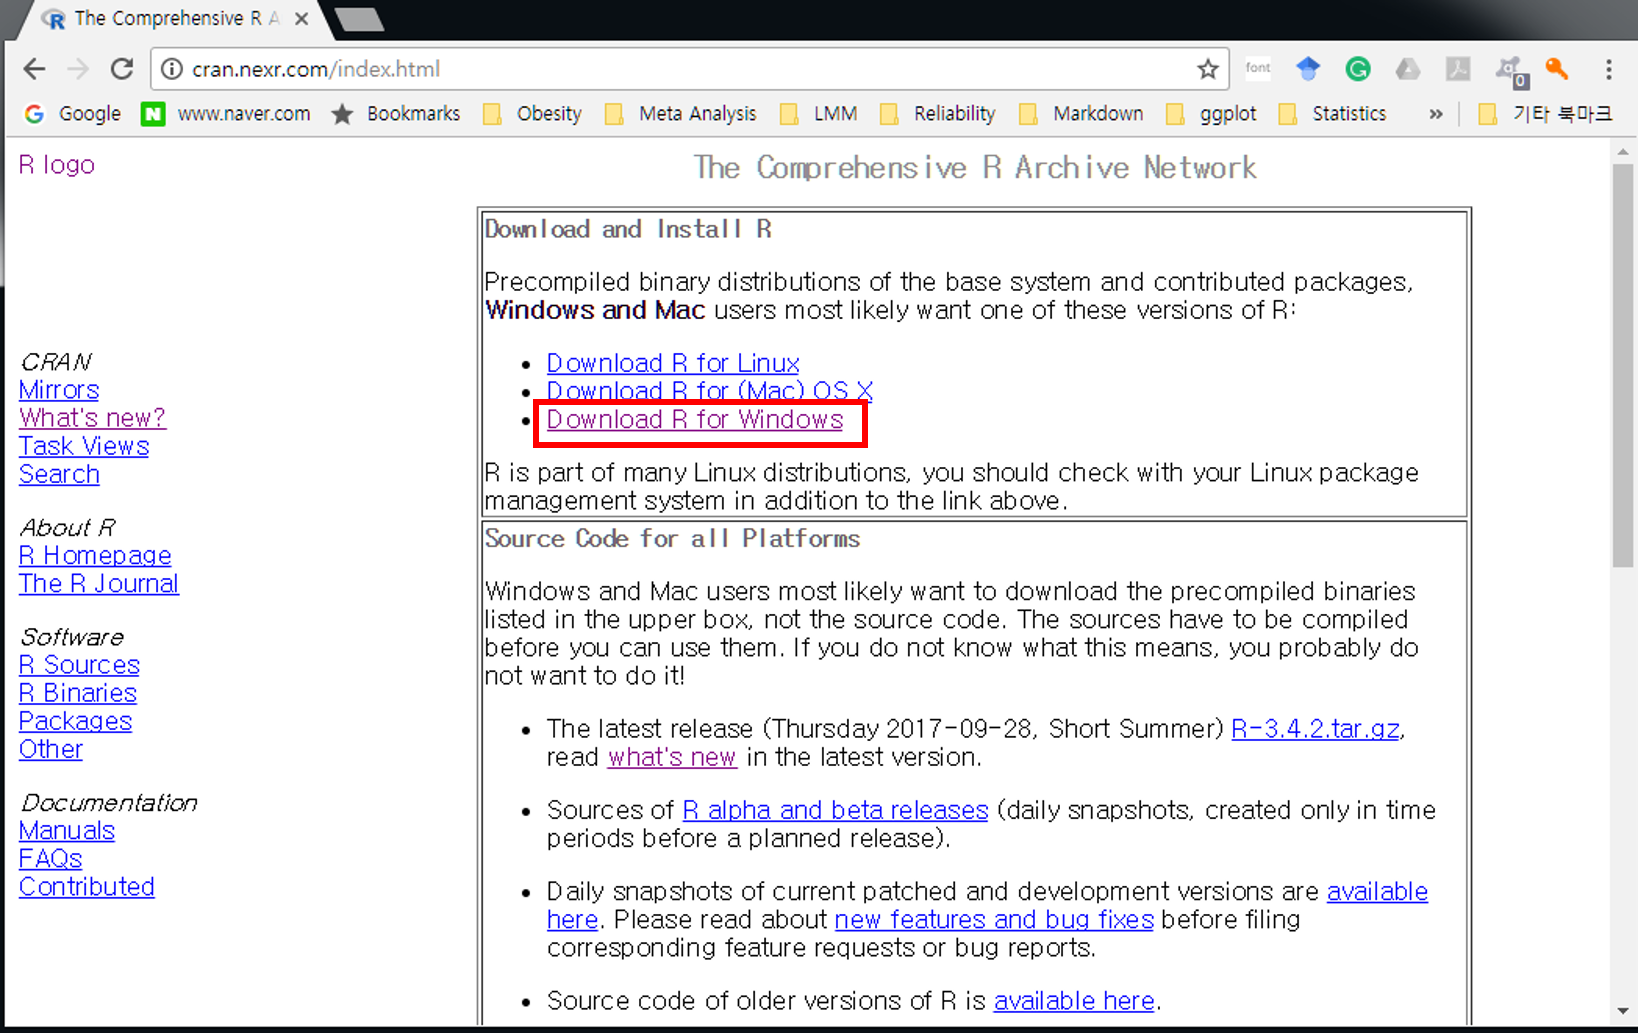
\includegraphics[width=0.9\linewidth]{figures/Rinstall-01} \end{center}

\normalsize

\begin{enumerate}
\def\labelenumi{\arabic{enumi}.}
\setcounter{enumi}{4}
\tightlist
\item
  \textbf{Downloads R for Windows} 링크 클릭하면 다음과 같은 화면으로 이동
\end{enumerate}

\footnotesize

\begin{center}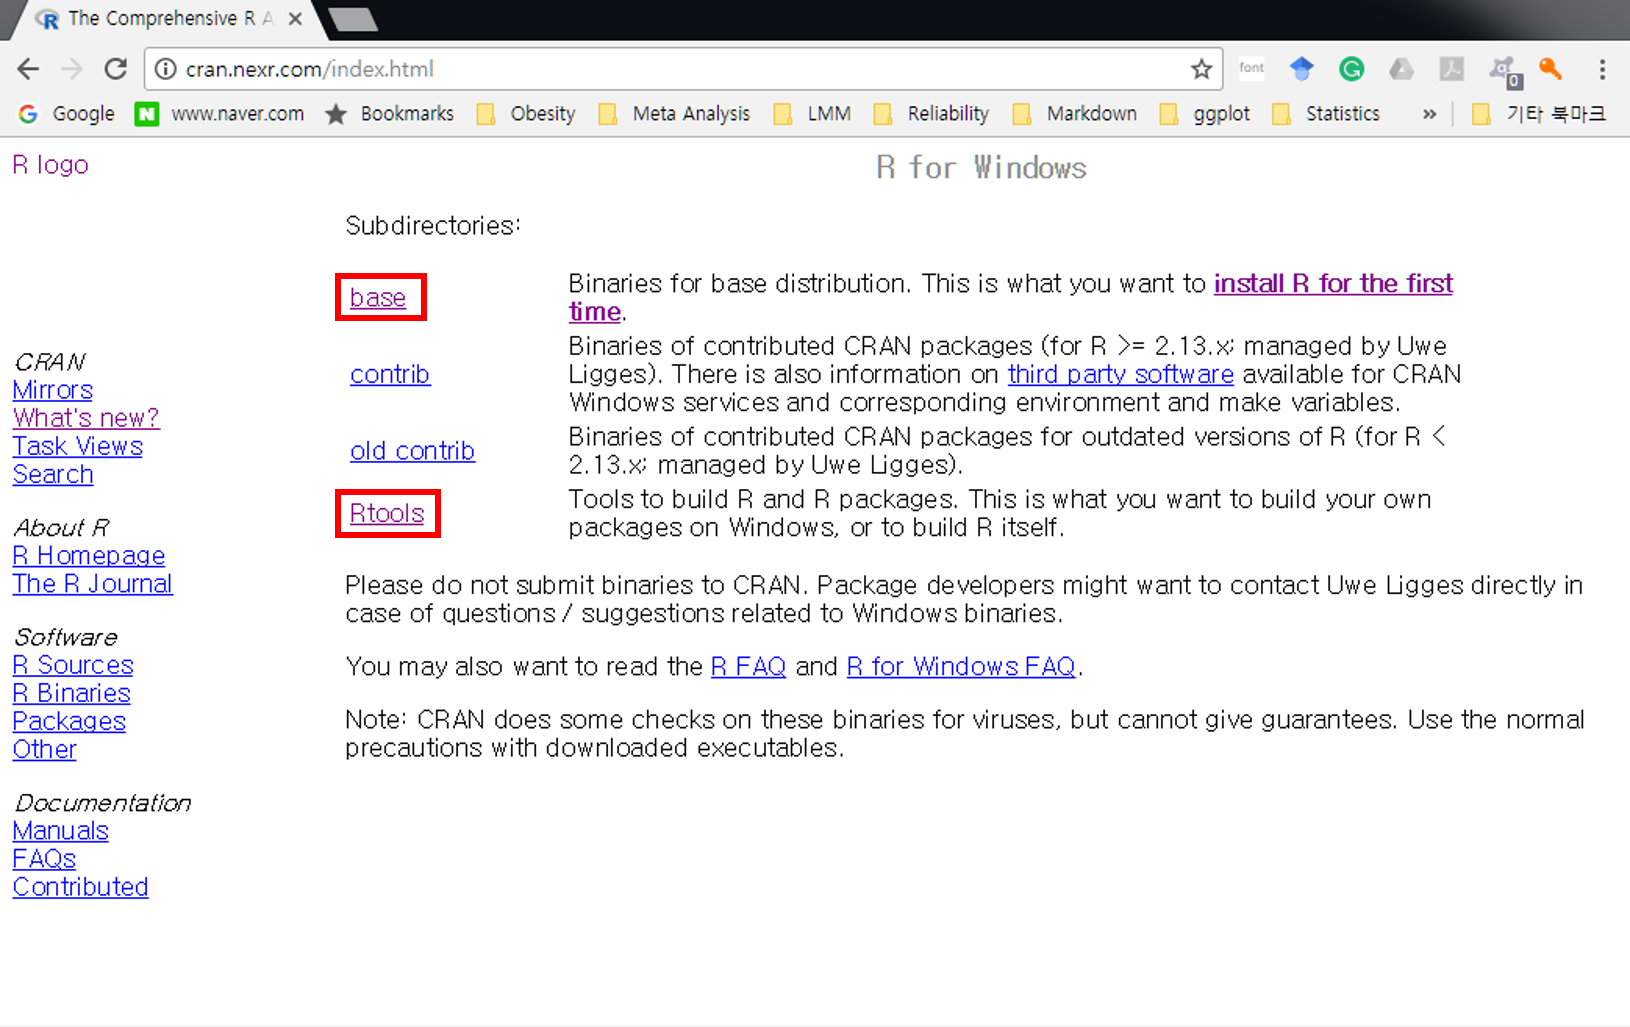
\includegraphics[width=0.9\linewidth]{figures/Rinstall-02} \end{center}

\normalsize

\footnotesize

\BeginKnitrBlock{rmdtip}
다음 하위폴더에 대한 간략 설멍

\begin{itemize}
\tightlist
\item
  \textbf{\texttt{base}}: R 실행 프로그램
\item
  \textbf{\texttt{contrib}}: R package의 바이너리 파일
\item
  \textbf{\texttt{Rtools}}: R package 개발 및 배포를 위한 프로그램
\end{itemize}
\EndKnitrBlock{rmdtip}

\normalsize

\begin{enumerate}
\def\labelenumi{\arabic{enumi}.}
\setcounter{enumi}{5}
\tightlist
\item
  위 화면에서 \textbf{base} 링크 클릭 후 아래 화면에서 \textbf{Downloads R 3.x.x for Windows} 를 클릭 후 설치 파일을 임의의 디렉토리에 저장 및 실행
\end{enumerate}

\footnotesize

\begin{center}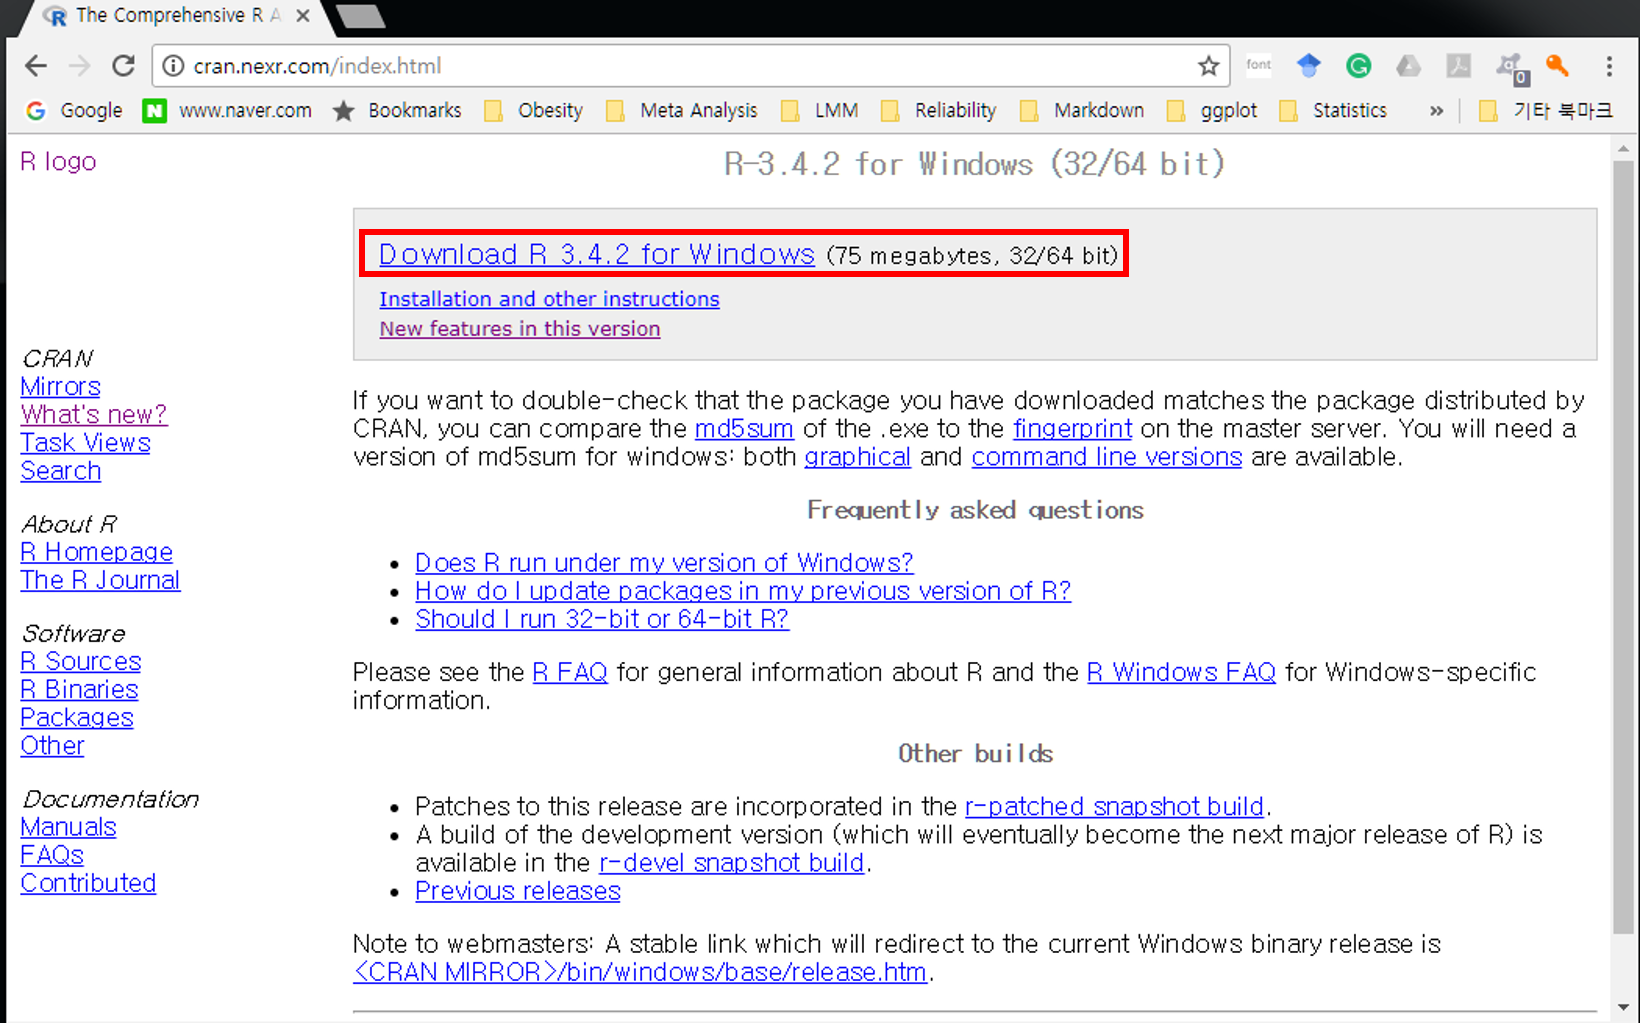
\includegraphics[width=0.9\linewidth]{figures/Rinstall-03} \end{center}

\normalsize

\begin{enumerate}
\def\labelenumi{\arabic{enumi}.}
\setcounter{enumi}{6}
\tightlist
\item
  다운로드한 파일을 실행하면 아래와 같은 대화창이 나타남

  \begin{itemize}
  \tightlist
  \item
    한국어 선택 \(\rightarrow\) 환영 화면에서 {[}다음(N)\textgreater{]} 클릭
  \end{itemize}
\end{enumerate}

\footnotesize

\begin{center}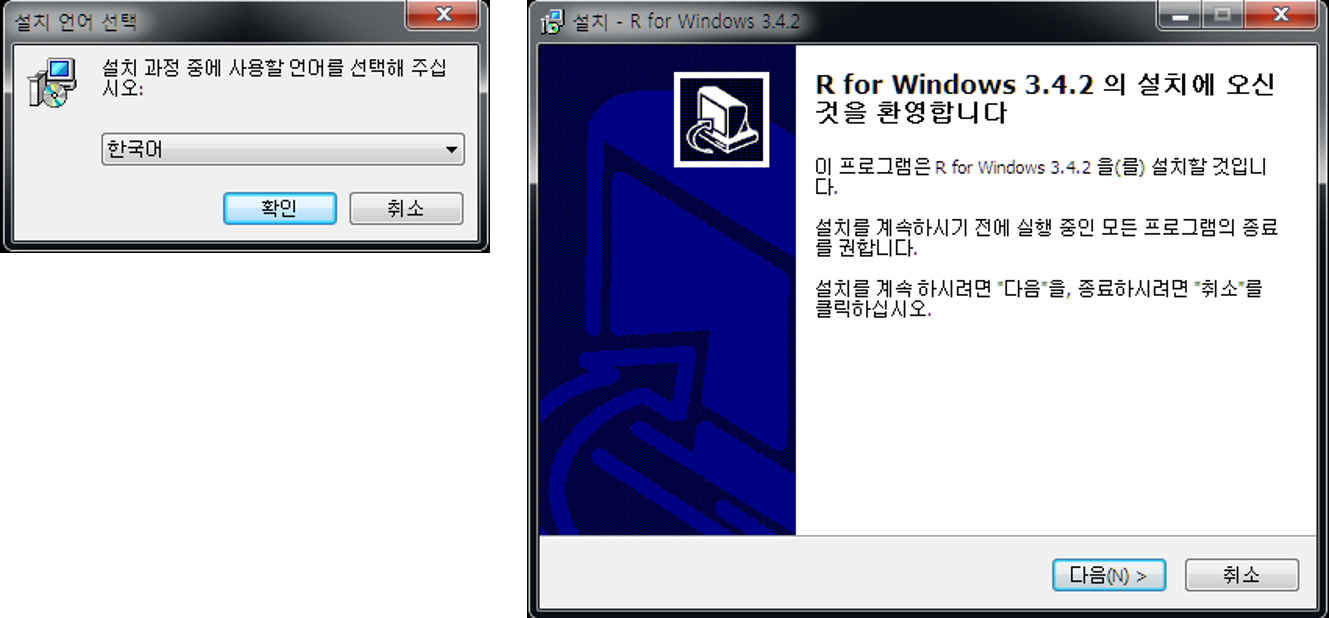
\includegraphics[width=0.9\linewidth]{figures/R-install-F01} \end{center}

\normalsize

\begin{enumerate}
\def\labelenumi{\arabic{enumi}.}
\setcounter{enumi}{7}
\tightlist
\item
  GNU 라이센스에 대한 설명 및 동의 여부({[}다음(N)\textgreater{]}) 클릭
\end{enumerate}

\footnotesize

\begin{center}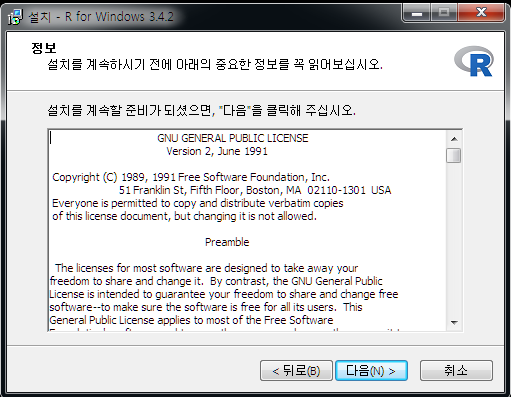
\includegraphics[width=0.9\linewidth]{figures/R-install-F02} \end{center}

\normalsize

\begin{enumerate}
\def\labelenumi{\arabic{enumi}.}
\setcounter{enumi}{8}
\tightlist
\item
  설치 디렉토리 설정 및 구성요소 설지 여부

  \begin{itemize}
  \tightlist
  \item
    원하는 디렉토리 설정(예: \texttt{C:\textbackslash{}R\textbackslash{}R-3.x.x})
  \item
    기본 프로그램(``Core Files''), 32 또는 64 bit 용 설치 파일, R console 한글 번역 모두 체크 뒤 {[}다음(N)\textgreater{]} 클릭
  \end{itemize}
\end{enumerate}

\footnotesize

\begin{center}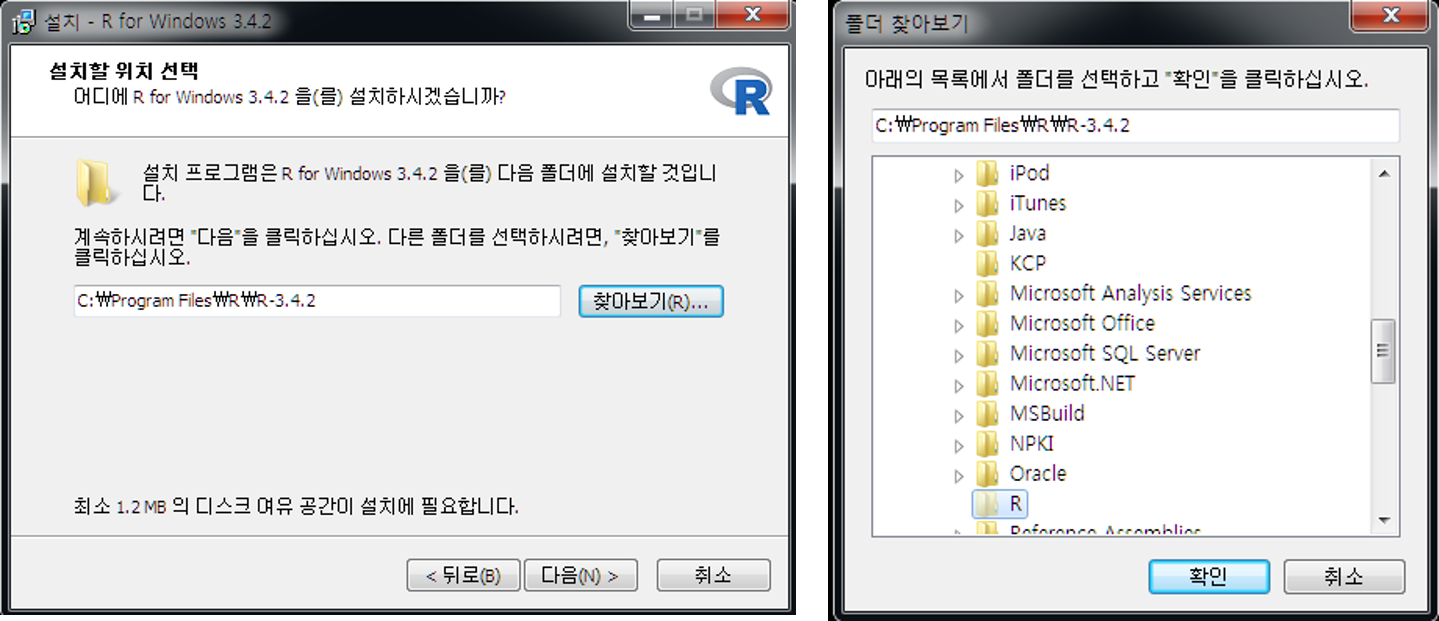
\includegraphics[width=0.9\linewidth]{figures/R-install-F03} \end{center}

\normalsize

\footnotesize

\begin{center}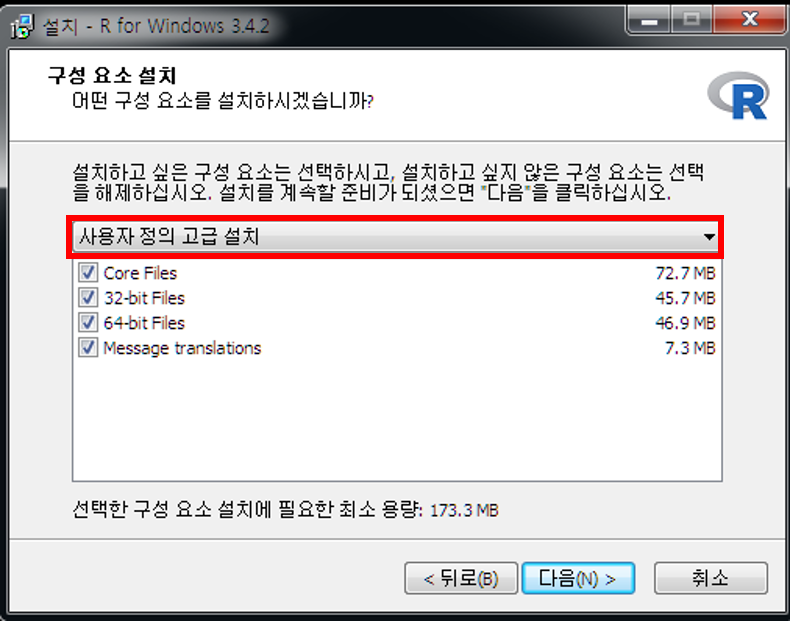
\includegraphics[width=0.9\linewidth]{figures/R-install-F04} \end{center}

\normalsize

\begin{enumerate}
\def\labelenumi{\arabic{enumi}.}
\setcounter{enumi}{9}
\tightlist
\item
  R 스타트업 옵션 지정
\end{enumerate}

\begin{itemize}
\tightlist
\item
  기본값(``No'' check-button)으로도 설치 진행 가능
\item
  본 문서에서는 스타트업 옵션 변경으로 진행
\end{itemize}

\footnotesize

\begin{center}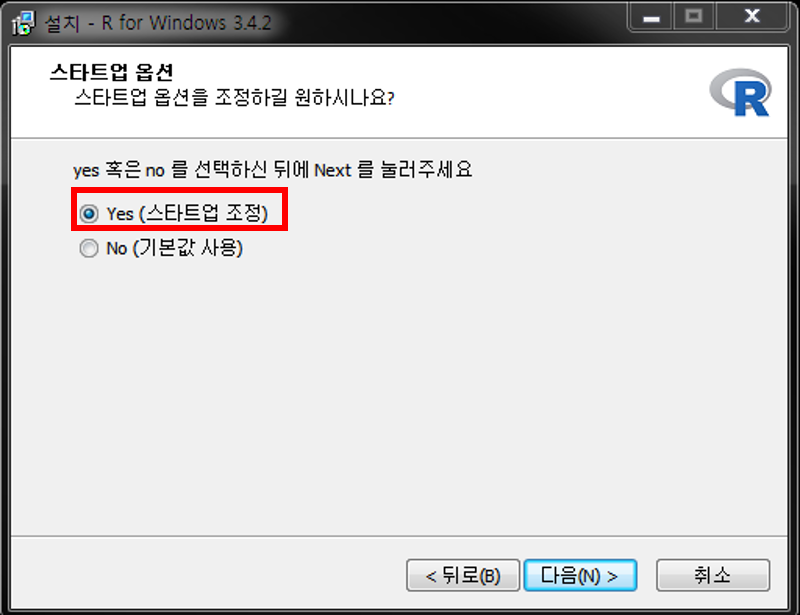
\includegraphics[width=0.9\linewidth]{figures/R-install-F05} \end{center}

\normalsize

\begin{enumerate}
\def\labelenumi{\arabic{enumi}.}
\setcounter{enumi}{10}
\tightlist
\item
  화면표시방식(디스플레이 모드) 설정 변경
\end{enumerate}

\begin{itemize}
\tightlist
\item
  MDI: 한 윈도우 내에서 script 편집창, 출력, 도움말 창 사용
\item
  SDI: 다중 창에서 각각 script 편집창, 출력, 도움말 등을 독립적으로 열기
\end{itemize}

\footnotesize

\begin{center}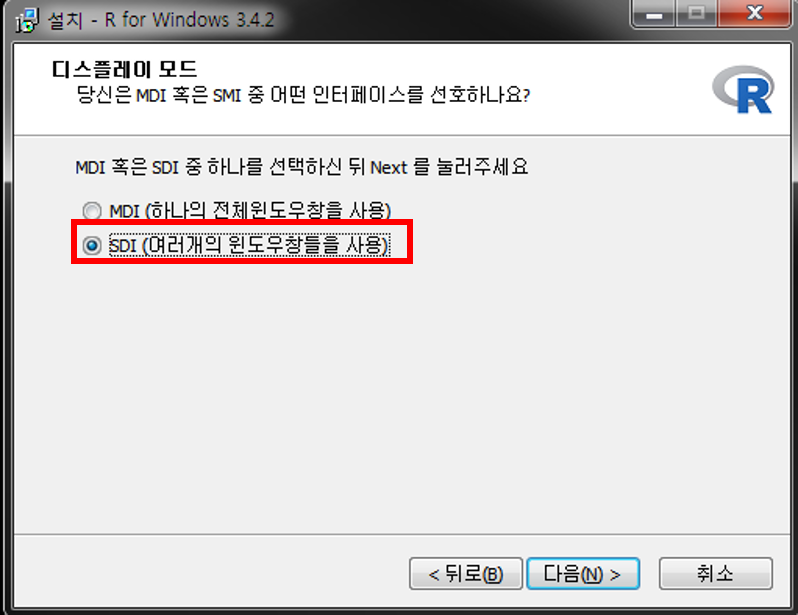
\includegraphics[width=0.9\linewidth]{figures/R-install-F06} \end{center}

\normalsize

\begin{enumerate}
\def\labelenumi{\arabic{enumi}.}
\setcounter{enumi}{11}
\tightlist
\item
  도움말 형식에서 HTML 도움말 기반 선택
\end{enumerate}

\footnotesize

\begin{center}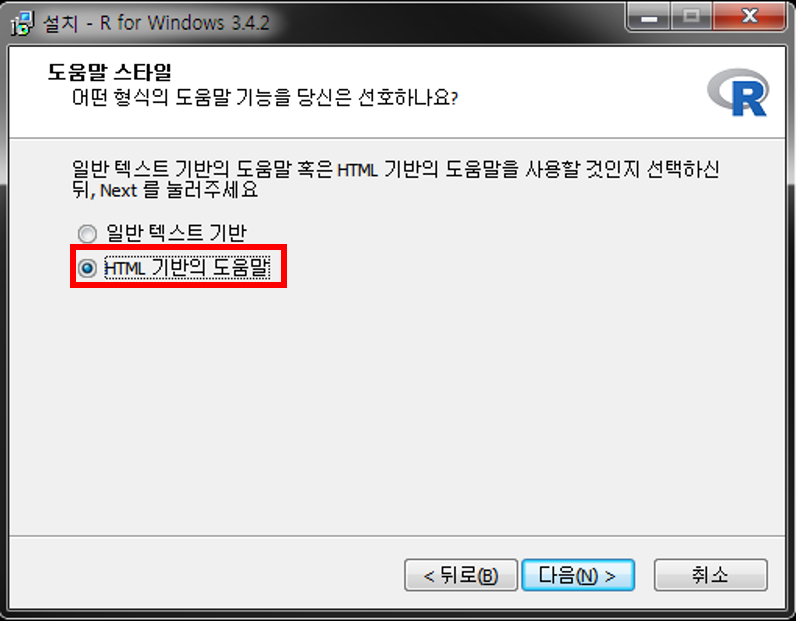
\includegraphics[width=0.9\linewidth]{figures/R-install-F07} \end{center}

\normalsize

\begin{enumerate}
\def\labelenumi{\arabic{enumi}.}
\setcounter{enumi}{12}
\tightlist
\item
  시작메뉴 폴더 선택
\end{enumerate}

\begin{itemize}
\tightlist
\item
  ``바로가기''를 생성할 시작 메뉴 폴더 지정 후 {[}다음(N)\textgreater{]} 클릭 후 설치 진행
\item
  하단 ``시작메뉴 폴더 만들지 않음'' 체크박스 표시 시 시작메뉴에 ``바로가기'' 아이콘이 생성되지 않음(실행에 전혀 지장 없음)
\end{itemize}

\footnotesize

\begin{center}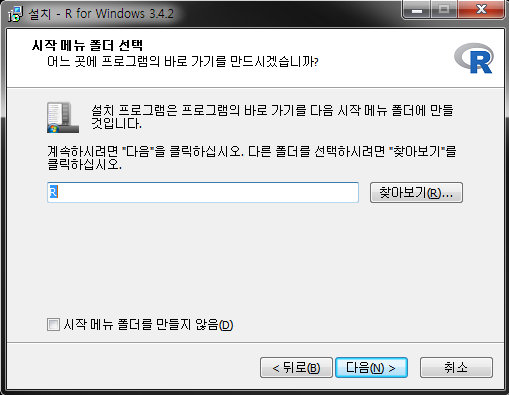
\includegraphics[width=0.9\linewidth]{figures/R-install-F08} \end{center}

\normalsize

\begin{enumerate}
\def\labelenumi{\arabic{enumi}.}
\setcounter{enumi}{13}
\tightlist
\item
  추가 옵션 지정: 바탕화면 아이콘 생성 등 추가적 작업 옵션 체크 후 {[}다음(N)\textgreater{]} 클릭 \(\rightarrow\) 설치 진행
\end{enumerate}

\begin{itemize}
\tightlist
\item
  설치된 R 버전 정보 레지스트리 저장 여부
\item
  \texttt{.Rdata} 확장자를 R 실행파일과 자동 연계
\end{itemize}

\footnotesize

\begin{center}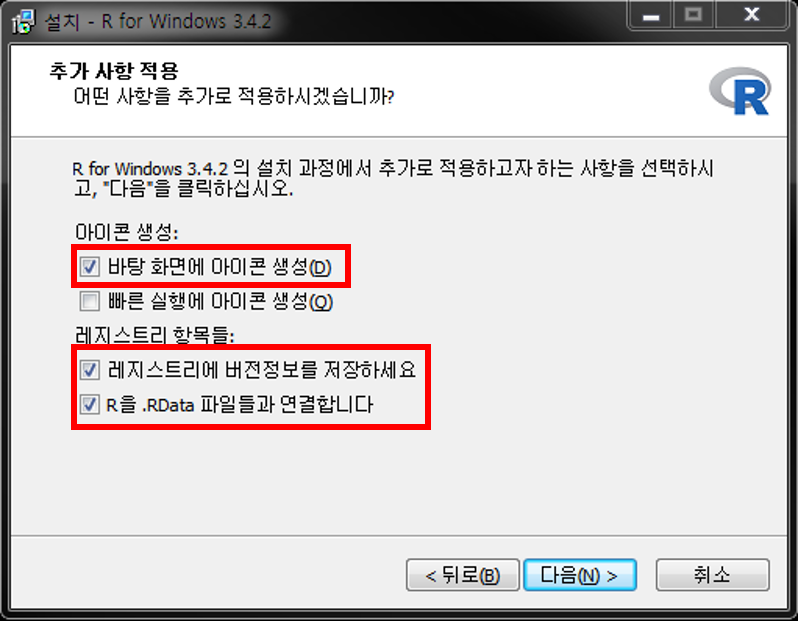
\includegraphics[width=0.9\linewidth]{figures/R-install-F09} \end{center}

\normalsize

\begin{enumerate}
\def\labelenumi{\arabic{enumi}.}
\setcounter{enumi}{14}
\tightlist
\item
  설치 완료 후 바탕화면의 R 아이콘을 더블클릭하면 Rgui가 실행
\end{enumerate}

\footnotesize

\begin{figure}

{\centering 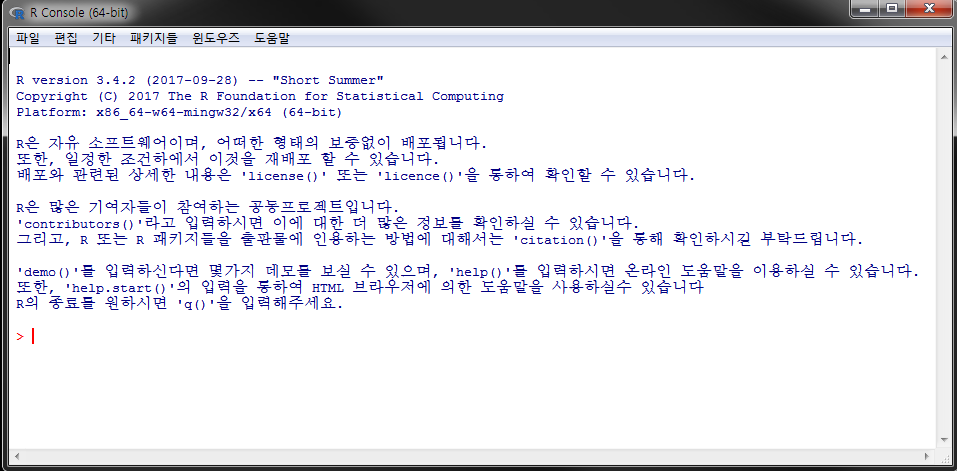
\includegraphics[width=1\linewidth]{figures/Rgui} 

}

\caption{Windows에서 R 실행화면(콘솔 창, SDI 모드)}\label{fig:r-console}
\end{figure}

\normalsize

\hypertarget{r-check}{%
\section{R 시작 및 작동 체크}\label{r-check}}

\BeginKnitrBlock{rmdimportant}
\textbf{실습}: 설치된 R을 실행 후 보이는 R 콘솔(consle) 창에서 명령어를 실행하고 결과 확인
\EndKnitrBlock{rmdimportant}

그림 Figure \ref{fig:r-console} 에서 \texttt{\textgreater{}} 기호는 R의 명령 프롬프트(prompt) 임

\begin{enumerate}
\def\labelenumi{\arabic{enumi}.}
\tightlist
\item
  현재 R session 정보(R 설치 버전, locale, 로딩 packages) 출력
\end{enumerate}

\footnotesize

\begin{Shaded}
\begin{Highlighting}[]
\CommentTok{# R의 설치 버전 및 현재 설정된 locale(언어, 시간대) 및 로딩된 R package 정보 출력}
\KeywordTok{sessionInfo}\NormalTok{() }
\end{Highlighting}
\end{Shaded}

\begin{verbatim}
R version 3.6.2 (2019-12-12)
Platform: x86_64-w64-mingw32/x64 (64-bit)
Running under: Windows 10 x64 (build 18363)

Matrix products: default

locale:
[1] LC_COLLATE=Korean_Korea.949  LC_CTYPE=Korean_Korea.949   
[3] LC_MONETARY=Korean_Korea.949 LC_NUMERIC=C                
[5] LC_TIME=Korean_Korea.949    

attached base packages:
[1] stats     graphics  grDevices utils     datasets  methods   base     

loaded via a namespace (and not attached):
 [1] compiler_3.6.2  magrittr_1.5    bookdown_0.16   tools_3.6.2    
 [5] htmltools_0.4.0 yaml_2.2.1      Rcpp_1.0.3      stringi_1.4.5  
 [9] rmarkdown_2.1   knitr_1.28      stringr_1.4.0   xfun_0.12      
[13] digest_0.6.25   rlang_0.4.5     evaluate_0.14  
\end{verbatim}

\normalsize

\begin{enumerate}
\def\labelenumi{\arabic{enumi}.}
\setcounter{enumi}{1}
\tightlist
\item
  문자열 출력
\end{enumerate}

\footnotesize

\begin{Shaded}
\begin{Highlighting}[]
\CommentTok{#문자열 출력}
\KeywordTok{print}\NormalTok{(}\StringTok{"Hello R"}\NormalTok{) }\CommentTok{#문자열}
\end{Highlighting}
\end{Shaded}

\begin{verbatim}
[1] "Hello R"
\end{verbatim}

\normalsize

\begin{quote}
\texttt{\#} 기호는 주석의 시작을 의미하고 실제로 실행되지 않음 같은 행에서 \texttt{\#} 뒤 내용의 코드 역시 실행되지 않음
\end{quote}

\begin{enumerate}
\def\labelenumi{\arabic{enumi}.}
\setcounter{enumi}{2}
\tightlist
\item
  \texttt{a} 라는 변수에 숫자 9, \texttt{b}라는 변수에 숫자 7를 할당 후 출력
\end{enumerate}

\footnotesize

\begin{Shaded}
\begin{Highlighting}[]
\CommentTok{# 수치형 값(scalar)을 변수에 할당(assign)}
\CommentTok{# 여러 명령어를 한줄에 입력할 때에는 세미콜론(;)으로 구분}
\NormalTok{a =}\StringTok{ }\DecValTok{9}\NormalTok{; b =}\StringTok{ }\DecValTok{7}
\NormalTok{a}
\end{Highlighting}
\end{Shaded}

\begin{verbatim}
[1] 9
\end{verbatim}

\begin{Shaded}
\begin{Highlighting}[]
\NormalTok{b}
\end{Highlighting}
\end{Shaded}

\begin{verbatim}
[1] 7
\end{verbatim}

\normalsize

\begin{enumerate}
\def\labelenumi{\arabic{enumi}.}
\setcounter{enumi}{3}
\tightlist
\item
  변수 \texttt{a}와 \texttt{b}의 사칙연산
\end{enumerate}

\footnotesize

\begin{Shaded}
\begin{Highlighting}[]
\NormalTok{a}\OperatorTok{+}\NormalTok{b; a}\OperatorTok{-}\NormalTok{b; a}\OperatorTok{*}\NormalTok{b; a}\OperatorTok{/}\NormalTok{b}
\end{Highlighting}
\end{Shaded}

\begin{verbatim}
[1] 16
\end{verbatim}

\begin{verbatim}
[1] 2
\end{verbatim}

\begin{verbatim}
[1] 63
\end{verbatim}

\begin{verbatim}
[1] 1.285714
\end{verbatim}

\normalsize

\begin{enumerate}
\def\labelenumi{\arabic{enumi}.}
\setcounter{enumi}{4}
\tightlist
\item
  R 그래픽 맛보기: 정규분포로부터 난수 100개 생성 후 생성된 데이터에 대한 히스토그램 작성
\end{enumerate}

\footnotesize

\begin{Shaded}
\begin{Highlighting}[]
\CommentTok{# 난수 생성 시 값은 매번 달라지기 때문에 seed를 주어 일정값이 생성되도록 고정}
\CommentTok{# "="과 "<-"는 모두 동일한 기능을 가진 할당 연산자임}
\CommentTok{#평균이 0 이고 분산이 1인 정규분포에서 난수 100개 생성}
\KeywordTok{set.seed}\NormalTok{(}\DecValTok{12345}\NormalTok{) }\CommentTok{# random seed 지정}
\NormalTok{x <-}\StringTok{ }\KeywordTok{rnorm}\NormalTok{(}\DecValTok{100}\NormalTok{) }\CommentTok{# 난수 생성}
\KeywordTok{hist}\NormalTok{(x) }\CommentTok{# 히스토그램}
\end{Highlighting}
\end{Shaded}

\begin{figure}

{\centering 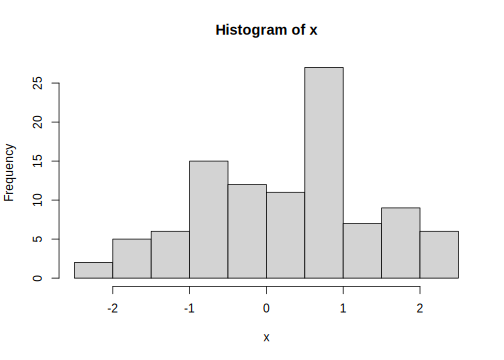
\includegraphics{01-overview_files/figure-latex/check-04-1} 

}

\caption{정규분포 100개의 히스토그램}\label{fig:check-04}
\end{figure}

\normalsize

\footnotesize

\BeginKnitrBlock{rmdtip}
R 명령어 또는 전체 프로그램 소스 실행 시 매우 빈번히 오류가 나타나는데, 이를 해결할 수 있는 가장 좋은 방법은 앞에서 언급한 Google을 이용한 검색 또는 R 설치 시 자체적으로 내장되어 있는 도움말을 참고하는 것이 가장 효율적임.
\EndKnitrBlock{rmdtip}

\normalsize

\footnotesize

\begin{table}[H]

\caption{\label{tab:tab-help}R help 관련 명령어 리스트}
\centering
\fontsize{10}{12}\selectfont
\begin{tabular}[t]{l>{\raggedright\arraybackslash}p{5cm}l}
\toprule
도움말 보기 명령어 & 설명 & 사용법\\
\midrule
\rowcolor{gray!6}  `help` 또는 `?` & 도움말 시스템 호출 & `help(함수명)`\\
`help.search` 또는 `??` & 주어진 문자열을 포함한 문서 검색 & `help.search(pattern)`\\
\rowcolor{gray!6}  `example` & topic의 도움말 페이지에 있는 examples section 실행 & `example(함수명)`\\
`vignette` & topic의 pdf 또는 html 레퍼런스 메뉴얼 불러오기 & `vignette(패키지명 또는 패턴)`\\
\bottomrule
\end{tabular}
\end{table}

\normalsize

\footnotesize

\BeginKnitrBlock{rmdtip}
\textbf{Vignette} 의 활용

\begin{itemize}
\tightlist
\item
  \texttt{vignette()}에서 제공하는 문서는 데이터를 기반으로 사용하고자 하는 패키지의 실제 활용 예시를 작성한 문서이기 때문에 초보자들이 R 패키지 활용에 대한 접근성을 높혀줌.
\item
  \texttt{browseVignettes()} 명령어를 통해 vignette을 제공하는 R 패키지 및 해당 vignette 문서 확인 가능
\end{itemize}
\EndKnitrBlock{rmdtip}

\normalsize

\hypertarget{rconsle-script}{%
\section{R script 편집기 사용}\label{rconsle-script}}

\BeginKnitrBlock{rmdimportant}
\textbf{실습}: R 설치 후 Rgui 에서 제공하는 편집기(R editor)에 명령어를 입력하고 실행
\EndKnitrBlock{rmdimportant}

설치된 R을 실행 후 상단 pull-down 메뉴에서 {[}\textbf{File}{]} \(\rightarrow\) {[}\textbf{새 스크립트}{]}를 선택하면 아래 그림과 같이 편집창(R 인스톨 시 SDI 옵션 기준)이 나타남

\footnotesize

\begin{center}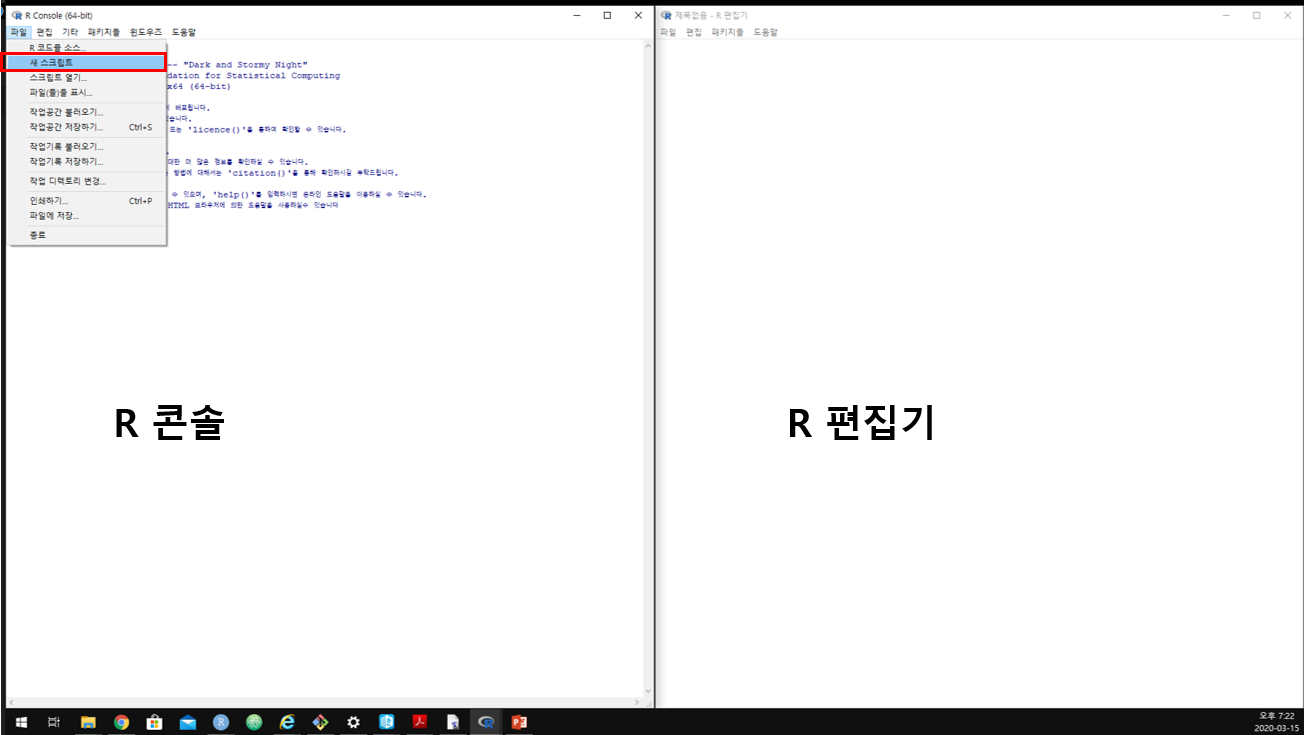
\includegraphics[width=1\linewidth]{figures/r-console-edit} \end{center}

\normalsize

편집기 창에 다음 명령어 입력

\footnotesize

\begin{Shaded}
\begin{Highlighting}[]
\CommentTok{# R에 내장된 cars 데이터셋 불러오기 cars dataset에 포함된 변수들의 기초통계량}
\CommentTok{# 출력 2차원 산점도}
\KeywordTok{data}\NormalTok{(cars)}
\KeywordTok{help}\NormalTok{(cars)  }\CommentTok{# cars 데이터셋에 대한 설명 help 창에 출력}
\KeywordTok{head}\NormalTok{(cars)  }\CommentTok{# cars 데이터셋 처음 6개 행 데이터 출력}
\KeywordTok{summary}\NormalTok{(cars)  }\CommentTok{# cars 데이터셋 요약}
\KeywordTok{plot}\NormalTok{(cars)  }\CommentTok{# 변수가 2개인 경우 산점도 출력}
\end{Highlighting}
\end{Shaded}

\normalsize

\begin{itemize}
\tightlist
\item
  편집창에서 한 줄을 실행시키려면 명령어가 입력된 줄에서 \textbf{{[}Ctrl{]}} + \textbf{{[}R{]}} 입력
\item
  편집창에 입력한 모든 명령어를 실행시키려면 모든 줄을 선택(마우스 또는 {[}Shift{]} + \(\downarrow\))
\end{itemize}

\footnotesize

\begin{verbatim}
  speed dist
1     4    2
2     4   10
3     7    4
4     7   22
5     8   16
6     9   10
\end{verbatim}

\begin{verbatim}
     speed           dist       
 Min.   : 4.0   Min.   :  2.00  
 1st Qu.:12.0   1st Qu.: 26.00  
 Median :15.0   Median : 36.00  
 Mean   :15.4   Mean   : 42.98  
 3rd Qu.:19.0   3rd Qu.: 56.00  
 Max.   :25.0   Max.   :120.00  
\end{verbatim}

\begin{figure}
\centering
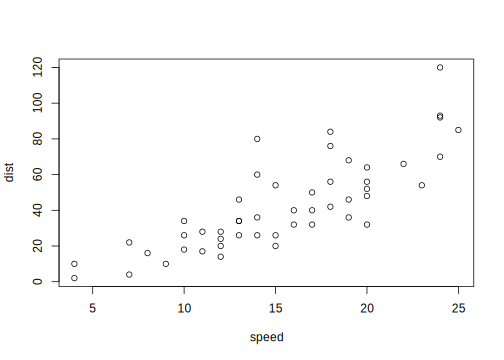
\includegraphics{01-overview_files/figure-latex/check-edit-out-1.pdf}
\caption{\label{fig:check-edit-out}cars 데이터셋의 speed와 dist 간 2차원 산점도: speed는 자동차 속도(mph)이고 dist는 해당 속도에서 브레이크를 밟았을 때 멈출 때 까지 걸린 거리(ft)를 나타냄.}
\end{figure}

\normalsize

\begin{itemize}
\tightlist
\item
  R은 명령어를 입력하고 실행결과를 확인하는 대화형(interpreter) 방식
\item
  콘솔창에서 \(\uparrow\)/\(\downarrow\)를 누르면 이전/이후 실행 명령 기록 확인 가능
\item
  여러 줄 이상 R 명령어라든가 반복적, 장기간 작업을 수행해야 할 경우 R 명령어로 구성된 스크립트 작성 후 일괄 실행하는 것이 일반적
\item
  여러 다중 명령 코딩 시 콘솔창에 직접 입력하는 것은 비효율적이므로 스크립트 에디터를 사용
\item
  위 예시처럼 R 에디터 사용할 수 있으나 가독성 및 코딩 효율이 떨어짐
\item
  과거 많이 사용됐던 R 에디터: \href{http://www.winedt.com}{WinEdt}, \href{https://sourceforge.net/projects/tinn-r/}{Tinn-R}, \href{http://www.vim.org/scripts/script.php?script_id=2628}{Vim}
\item
  현재 가장 범용적 R 에디터: \textbf{Rstudio}
\end{itemize}

\hypertarget{r-studio}{%
\section{RStudio}\label{r-studio}}

\begin{itemize}
\tightlist
\item
  \href{https://rstudio.com/}{RStudio}: R 통합 분석/개발 환경(integrated development environment, IDE)으로 현재 가장 대중적으로 사용되고 있는 R 사용 환경
\item
  명령 곤솔 외 파일 편집, 데이터 객체, 명령 기록(.history), 그래프 등에 쉽게 접근 가능
\item
  RStudio 독자적인 개발 환경 제공: Rmarkdown, Rnotebook, Shiny Web Application 등 다양한 R 환경을 제공
\item
  버전관리(git, subversion)를 통해 project 관리 가능
\item
  \textbf{무료} 및 유료 소프트웨어 제공
\end{itemize}

\hypertarget{rstudio-install}{%
\subsection{RStudio 설치하기}\label{rstudio-install}}

\begin{enumerate}
\def\labelenumi{\arabic{enumi}.}
\tightlist
\item
  웹 브라우저를 통해 \url{https://rstudio.com} 접속 후 상단 \href{https://rstudio.com/products/rstudio/download/}{DOWNLOAD} 링크 클릭
\end{enumerate}

\footnotesize

\begin{center}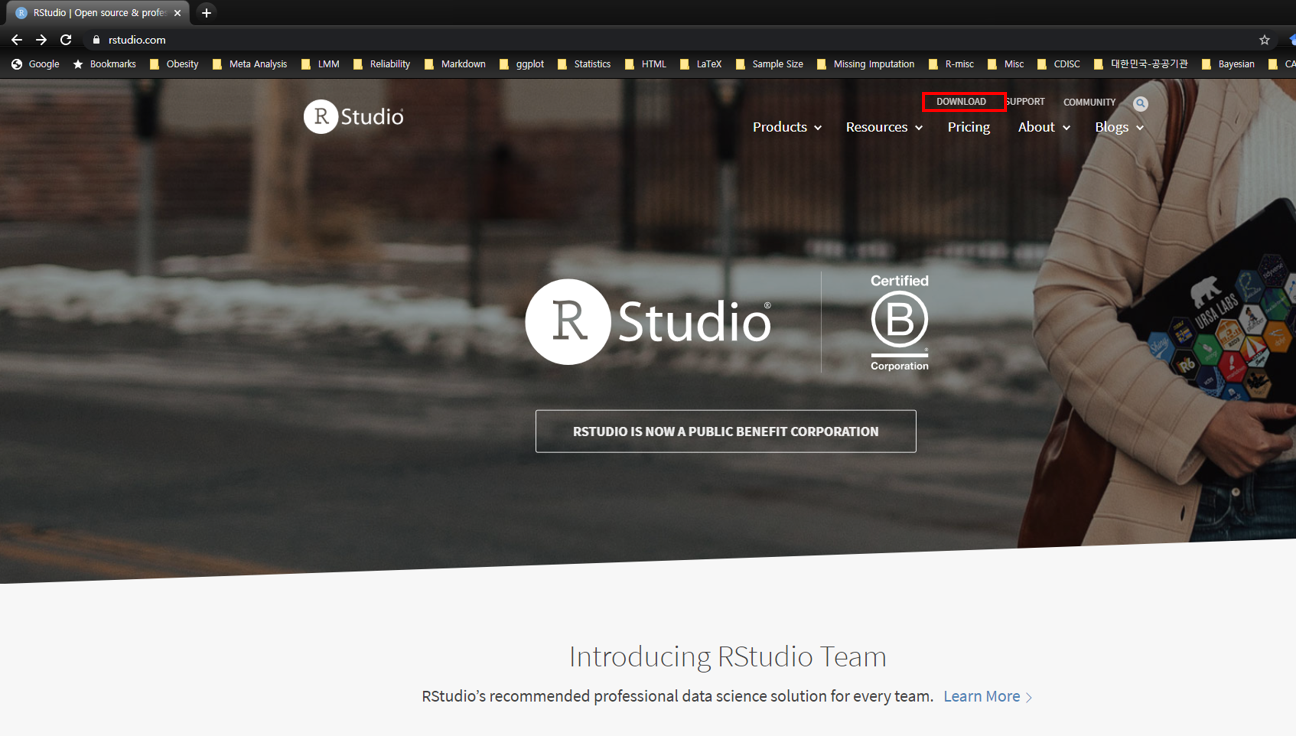
\includegraphics[width=1\linewidth]{figures/rstudio-homepage} \end{center}

\normalsize

\begin{enumerate}
\def\labelenumi{\arabic{enumi}.}
\setcounter{enumi}{1}
\item
  Desktop 또는 Server 버전 중 택일

  \begin{itemize}
  \tightlist
  \item
    서버용 설치를 위해서는 Server 클릭 \(\rightarrow\) 소규모 자료 분석용으로는 불필요
  \item
    여기서는 \textbf{Desktop} 버전 선택 후 다음 링크로 이동
  \end{itemize}
\end{enumerate}

\footnotesize

\begin{center}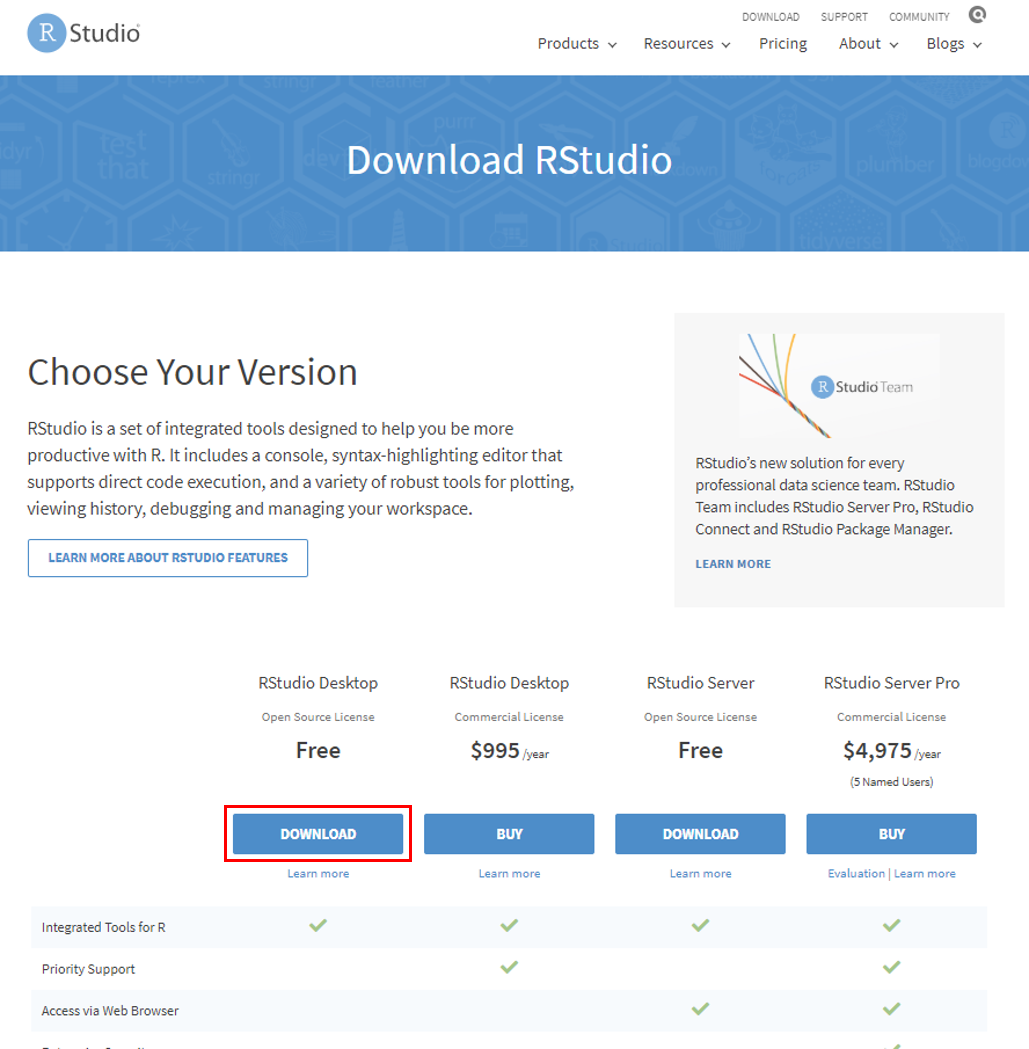
\includegraphics[width=1\linewidth]{figures/rstudio-download} \end{center}

\normalsize

\begin{enumerate}
\def\labelenumi{\arabic{enumi}.}
\setcounter{enumi}{2}
\tightlist
\item
  운영체제에 맞는 Rstudio installer 다운로드(여기서는 Windows 버전 다운로드)
\end{enumerate}

\footnotesize

\begin{center}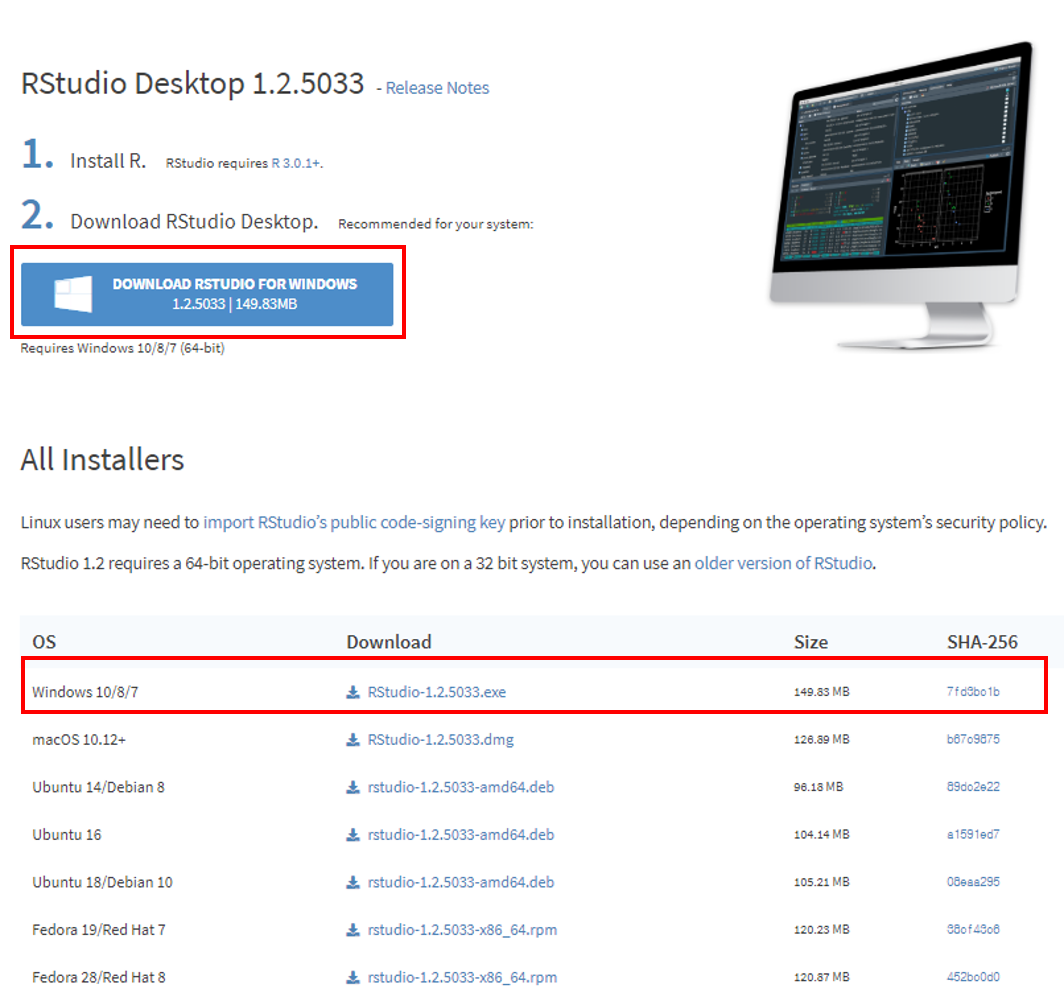
\includegraphics[width=1\linewidth]{figures/r-studio-download-02} \end{center}

\normalsize

\begin{enumerate}
\def\labelenumi{\arabic{enumi}.}
\setcounter{enumi}{3}
\tightlist
\item
  RStudio installer 다운로드 시 파일이 저장된 폴더에서 보통 \texttt{RStudio-xx.xx.xxx.exe} 형식의 파일명 확인

  \begin{itemize}
  \tightlist
  \item
    더블 클릭 후 실행
  \item
    \textbf{{[}다음\textgreater{]}} 몇 번 클릭 후 설치 종료
  \end{itemize}
\end{enumerate}

\footnotesize

\begin{center}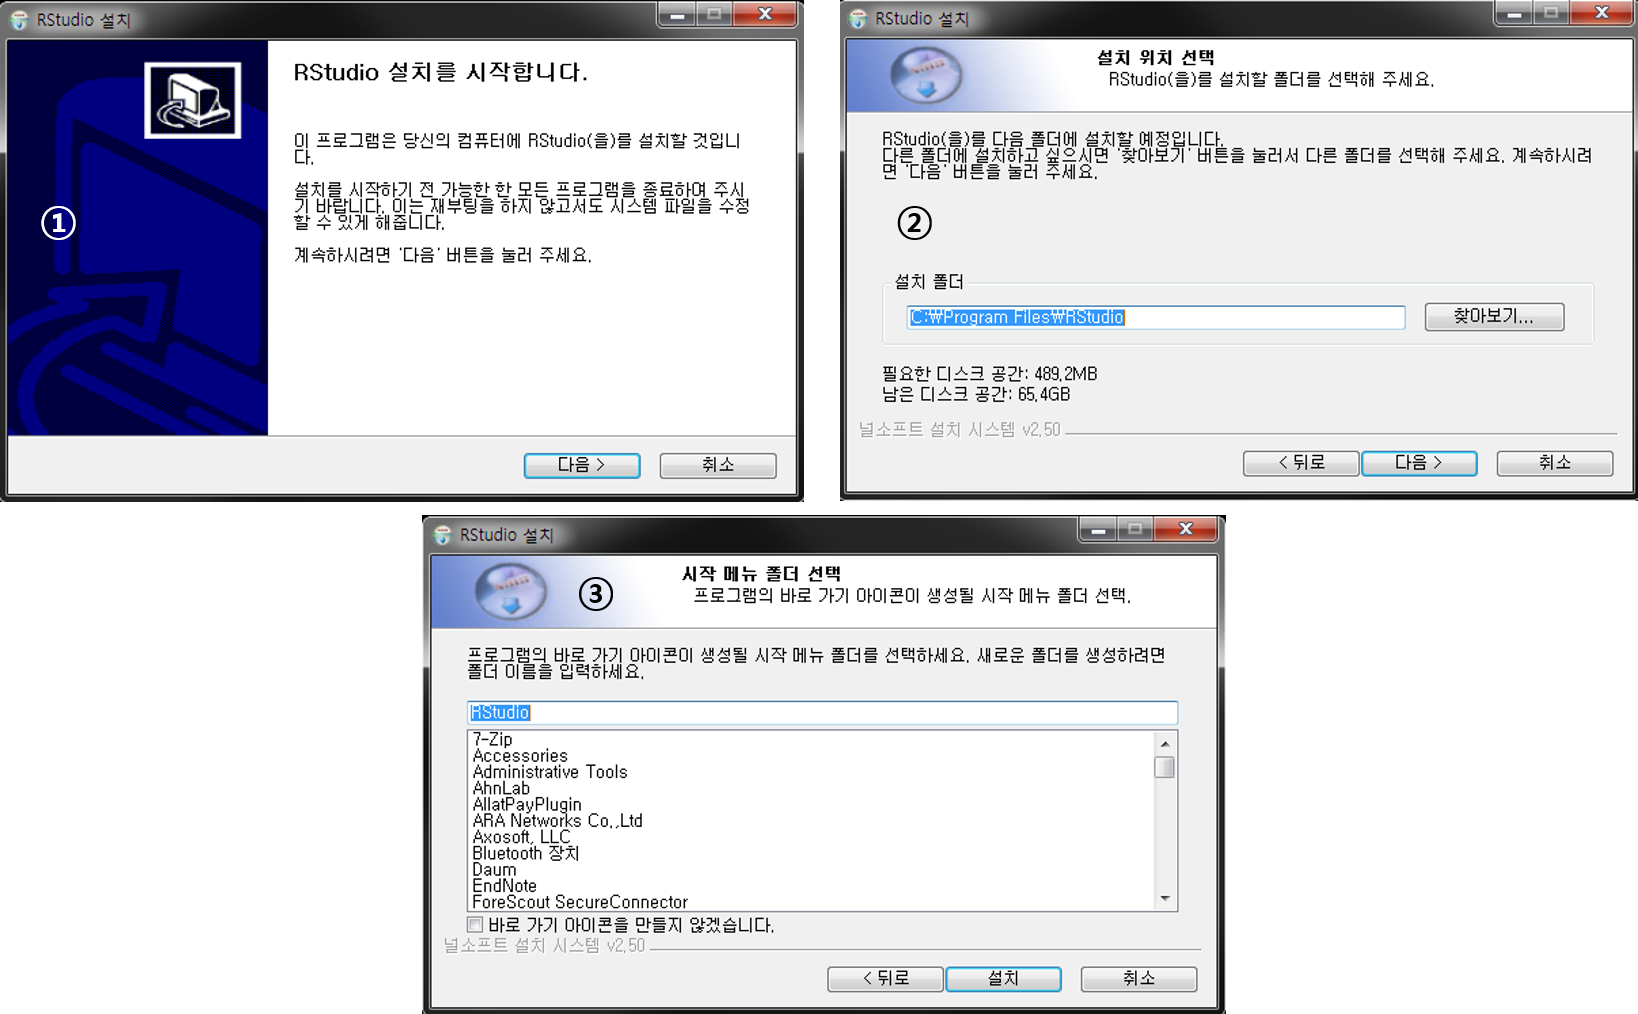
\includegraphics[width=1\linewidth]{figures/Rstudio-installer} \end{center}

\normalsize

  \bibliography{book.bib,packages.bib}

\printindex

\end{document}
